\documentclass[12pt]{cornelltfpxsop}
\title{DEE construction: Gluing  parts into DEE mechanical structure}
\date{September 13, 2024}
\author{M.Acero,T.Babenko,J.Monroy}
\approved{Jose Monroy}

\usepackage{paracol}
\setlength{\columnseprule}{0.4pt}

\sopid{DC}
\sopversion{v1}
\sopabstract{Describes the procedures to glue co-cured Carbon fiber-foam halves housing PEEK inserts, and titanium flower pattern evaporator, using the robotic gantry. The procedure takes place in the clean room. This is a two-person procedure.}



\begin{document}

\maketitle
%------------------------------------------------------------------
\section{Scope}
This is a regular part in the integration process of the TFPX cartridge.

%------------------------------------------------------------------
\section{Purpose}
The ``DEE'' is the mechanical structure supporting the silicon modules. It also provides cooling and support for power cables and e-links.    

%------------------------------------------------------------------
\section{Definitions}

\begin{itemize}
    \item Motion Composer: is a program that runs GCODE. GCODE is a set of instructions for the Gantry to move along. Think of a GCODE path like the path a paintbrush needs to be moved along to make a painting.
    %\item For all the GCODE programs, there is a delay of about 5 seconds to allow user to position near the NPaq switch just in case.
    
    \item Flower Pattern: The cooling tube or evaporator has a flower shape which we call here flower pattern. The Gantry needs to deposit epoxy while it is moving along the flower pattern path in the Dee. For this, we have a GCODE script/program run by Motion composer. LabView program "depositwhilemoving", ONLY deposit epoxy while the Gantry is being moved by Motion Composer in the flower pattern.

    \item Carbon fiber-foam co-cure (CFF): The DEE structure is formed by two skins of carbon fiber and two bodies of carbon foam. One carbon fiber skin and carbon foam are co-cured in one entity, so that the DEE is composed of 2 halves of CFF (CFF\_A and CFF\_B). In between the two CFF, inserts and evaporator are sandwiched.    
    
    \item Insert Filling: DEE has some PEEK inserts that will serve as clamping points for structures/objects on it. The Gantry moves to the location of the insert holes and deposit epoxy while STOPPED at that position. 
    
    \item Front panel: It is the window through which the user interact with the software. It show statistical information, status of the vacuum system, tools and elements in use and other information.  NOTE: put a pic of the front panel for reference!!!!! 
    \begin{center}
\begin{figure}[h!]
\includegraphics[width=0.8\textwidth]{img/Front_Panel.png}
\caption{Front Panel of DEE_ASSEMBLY_MASTER.vi}
\label{gantry_setup}
\end{figure}
\end{center}
\end{itemize}

%------------------------------------------------------------------
%\section{Responsibilities}

%------------------------------------------------------------------
\section{Equipment}
\begin{center}
\begin{figure}[h!]
\includegraphics[width=0.8\textwidth]{img/gantryEpoxyLabeled.png}
\caption{Gantry setup. Labels indicate the main parts of the setup.}
\label{gantry_setup}
\end{figure}
\end{center}

\begin{enumerate}

\item Gantry (check that everything (labeled in the figure  \ref{gantry_setup}) is installed and working properly. 
    \begin{itemize}
        \item Syringe holder 
        \item Stands with alignment screws
        \item Pressurised air Dispenser - Ultimus II
        \item Vacuum manifold and lines.
        \item Gantry head camera with light
    \end{itemize}
\item Parts and tools
\begin{center}
\begin{figure}[h]
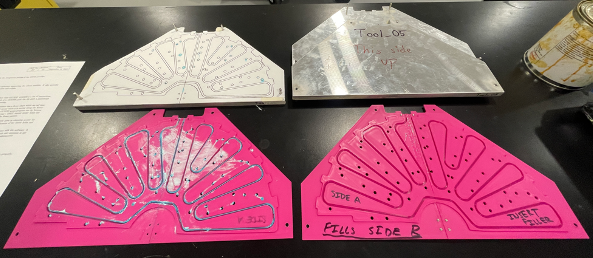
\includegraphics[width=0.45\textwidth,angle = 0]{img/PartsTools_1.png}
\includegraphics[width=0.45\textwidth,angle = 0]{img/PartsTools_2.png}\\
\includegraphics[width=0.45\textwidth,angle = 0]{img/centrifuge_TFPX.png}
\caption{Parts and tools used in the DEE manufacturing process. Materials listed for epoxy preparation should be located on the table inside room PSB 375 where the epoxy mixing will be performed; the rest of materials must be located on the table in front of the gantry except for evaporator, inserts and tweezers which should be located on the table left to the gantry.}
\label{Parts ands tools}
\end{figure}
\end{center}
    \begin{itemize}
        \item Side A Half-Dee CFF\_A 
        \item Side B Half-Dee CFF\_B
        \item PEEK Periphery
        \item EA9394 Epoxy  parts A and B. 
        \item Flower-Pattern Shape Titanium $CO_2$ tube/evaporator
        \item Box with PEEK inserts (56 will be used)
        \item Tweezers
        \item Two bottom jig plates
        \item One top jig plate
    \end{itemize}
\item Epoxy preparation \textbf{(Performed in PSB 375)}
    \begin{itemize}
        \item Bag of 12-20 Micron Diamond Powder
        \item EA9394 Epoxy Part A
        \item EA9394 Epoxy Part B
        \item 2 Popsicle Sticks
        \item Large Syringe, Piston, Cap, Olive Needle tip, Blue stopper cap
        \item Digital Scale
        \item Large Centrifuge with Counterweights Installed
        \item Paper Towels
        \item Isopropyl Alcohol
        \item Rubber beakers
        \item Silicone Gloves
        \item N95 Mask
        \item Extension cord
        \item Square plastic sheet
        \item Stopwatch
        \item Box Fan
        \item Mylar Plastic sheet
        \item Painter's Tape
        \item Small soft paint brush
    \end{itemize}
\end{enumerate}
%------------------------------------------------------------------

\section{Procedure}
\begin{paracol}{2} % Begin two-column layout  

\subsubsection*{Person 1:}

\begin{enumerate}
    %Perform a readiness check of the gantry:
%    \begin{itemize}[leftmargin=*]
    \item Check that the NPaq, power supplies, dispenser and vacuum pumps are\\turned on.
    \item Check compressed air lines are open
    \item Open LabView control software ``\textbf{C:\Users\co2_ctl\Documents\Final_Dee_Assembly\Labview\FINAL_DEE_ASSEMBLY_MASTER.vi}''. Make sure it is opened with Labview 2024.
    \item Open Motion composer
    \item Check that no other Gscript or Labview programs are running since they can interfere with the deposition.
    \item Test presence of vacuum.        
    \item Identify parts. Handle with gloves, face mask. Check that the parts are in good condition.
    \item Assign a new unique DEE number(\texttt{Dxxx}).
    \item Run the control software \textbf{FINAL_DEE_ASSEMBLY_MASTER.vi} and provide the information required:
    \begin{enumerate}
        \item Part numbers.
        \item DEE identification.
        \item other required info
    \end{enumerate}
    \item Mount the bottom jig plate onto the stand 1 and align it using the alignment screws(Figure \ref{JigAlignment}). Repeat for second bottom jig plate onto stand 2.
    \begin{figure}
        \centering
        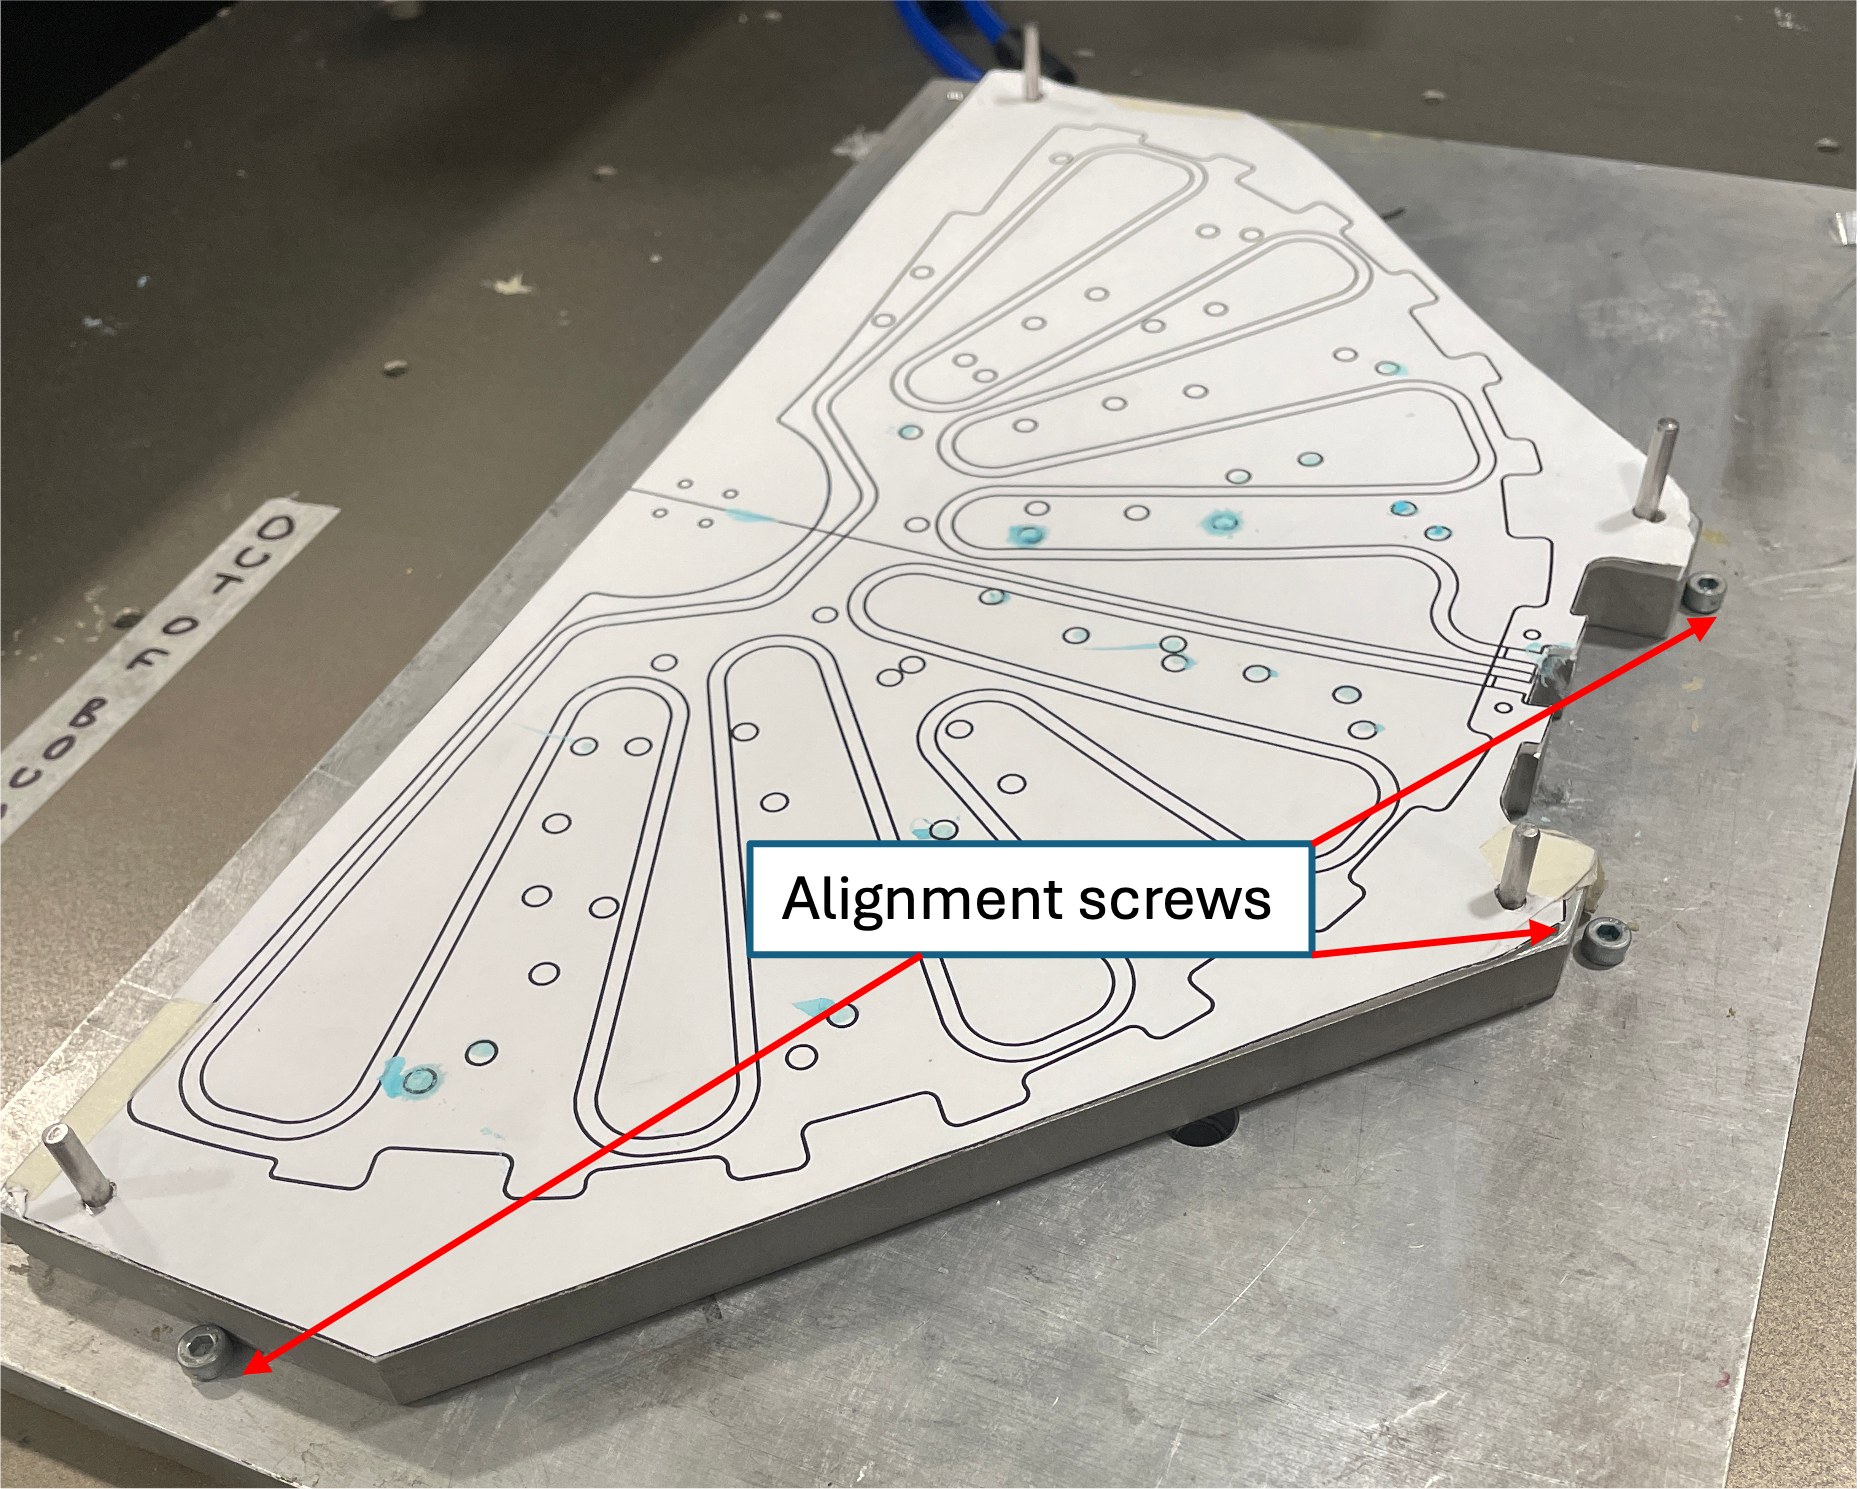
\includegraphics[width=0.8\linewidth]{img/jig_alignment.png}
        \caption{Jig alignment}
        \label{JigAlignment}
    \end{figure}
    \item Mount the CFF\_A onto the bottom jig plate on Stand 1 using the jig poles and holes in the CFF\_A. Repeat for CFF\_B on the bottom jig on stand 2.
    \item Put a rubber beaker on the scale and tare. Pour 8.1 g of Part A EA9396 epoxy in the beaker. Tare it again. Pour 2.4 g of part B EA9396 epoxy. Mix thoroughly for 2 minutes.   
    \item Spread plain epoxy on the PEEK periphery bottom face, using the paint brush.
    \item glue the Periphery to CFF\_A. Put some pressure around the periphery to ensure bonding. Use your hand/fingers 
    \item wait for Person 2 to bring the epoxy syringe into the clean room
 %   \end{itemize}

    %Gantry Loading, calibration and epoxy deposition
%    \begin{itemize}[leftmargin=*]
        \item Screw the blue pressure cap and hose assembly onto the syringe.
        \item Unscrew the blue stopper cap at the bottom of the syringe, install the needle tip and load the syringe into the syringe holder.
        \item Set the pressure at 35 psi. Make sure that after 20 minutes from this point, the pressure is adjusted to 45psi.
        \item check that the needle tip is in the starting point for epoxy deposition as shown in figure \ref{needleref}. If needle tip is not in position, adjust it using motion composer interface.
        \begin{figure}[h!]
            \centering
            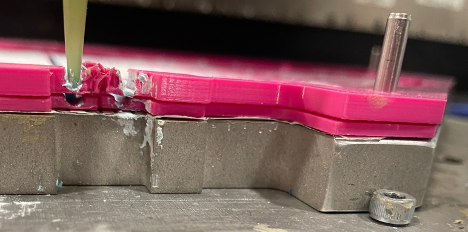
\includegraphics[width=0.45\linewidth]{img/NeedleRef.png}
            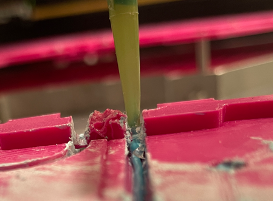
\includegraphics[width=0.45\linewidth]{img/NeedleRef2.png}
            \caption{Needle stating position}
            \label{needleref}
        \end{figure}
        \item Begin epoxy deposition by hitting OK button in the front panel of LabView program. Check for consistent epoxy flow. When deposition ends on CCF\_A, gantry will move to starting point on CFF\_B.  
        \item Check that the needle tip is in the starting point for epoxy deposition. Adjust accordingly. 
        \item Begin epoxy deposition by hitting OK button in the front panel of LabView program. Check for consistent epoxy flow.
%    \end{itemize}
    %Final DEE structure assembly.
%    \begin{itemize}
        \item Remove CFF\_B from Stand 2 and move it to working table on the left of the gantry. Bottom jig from stand 1 should already be on the table ready for stacking. 
        \item Flip CFF\_B so that carbon foam face towards the floor.
        \item Use poles on bottom jig to stack CFF\_B on top of CFF\_A.
        \item stack top jig plate on top of CFF\_B. Make sure everything fits.
        \item Take the full stack into the oven; turn on the oven and let bake for 2 hours. Follow instructions fixed on the oven door as shown in the figure \ref{oven}. 
        \begin{figure}
            \centering
            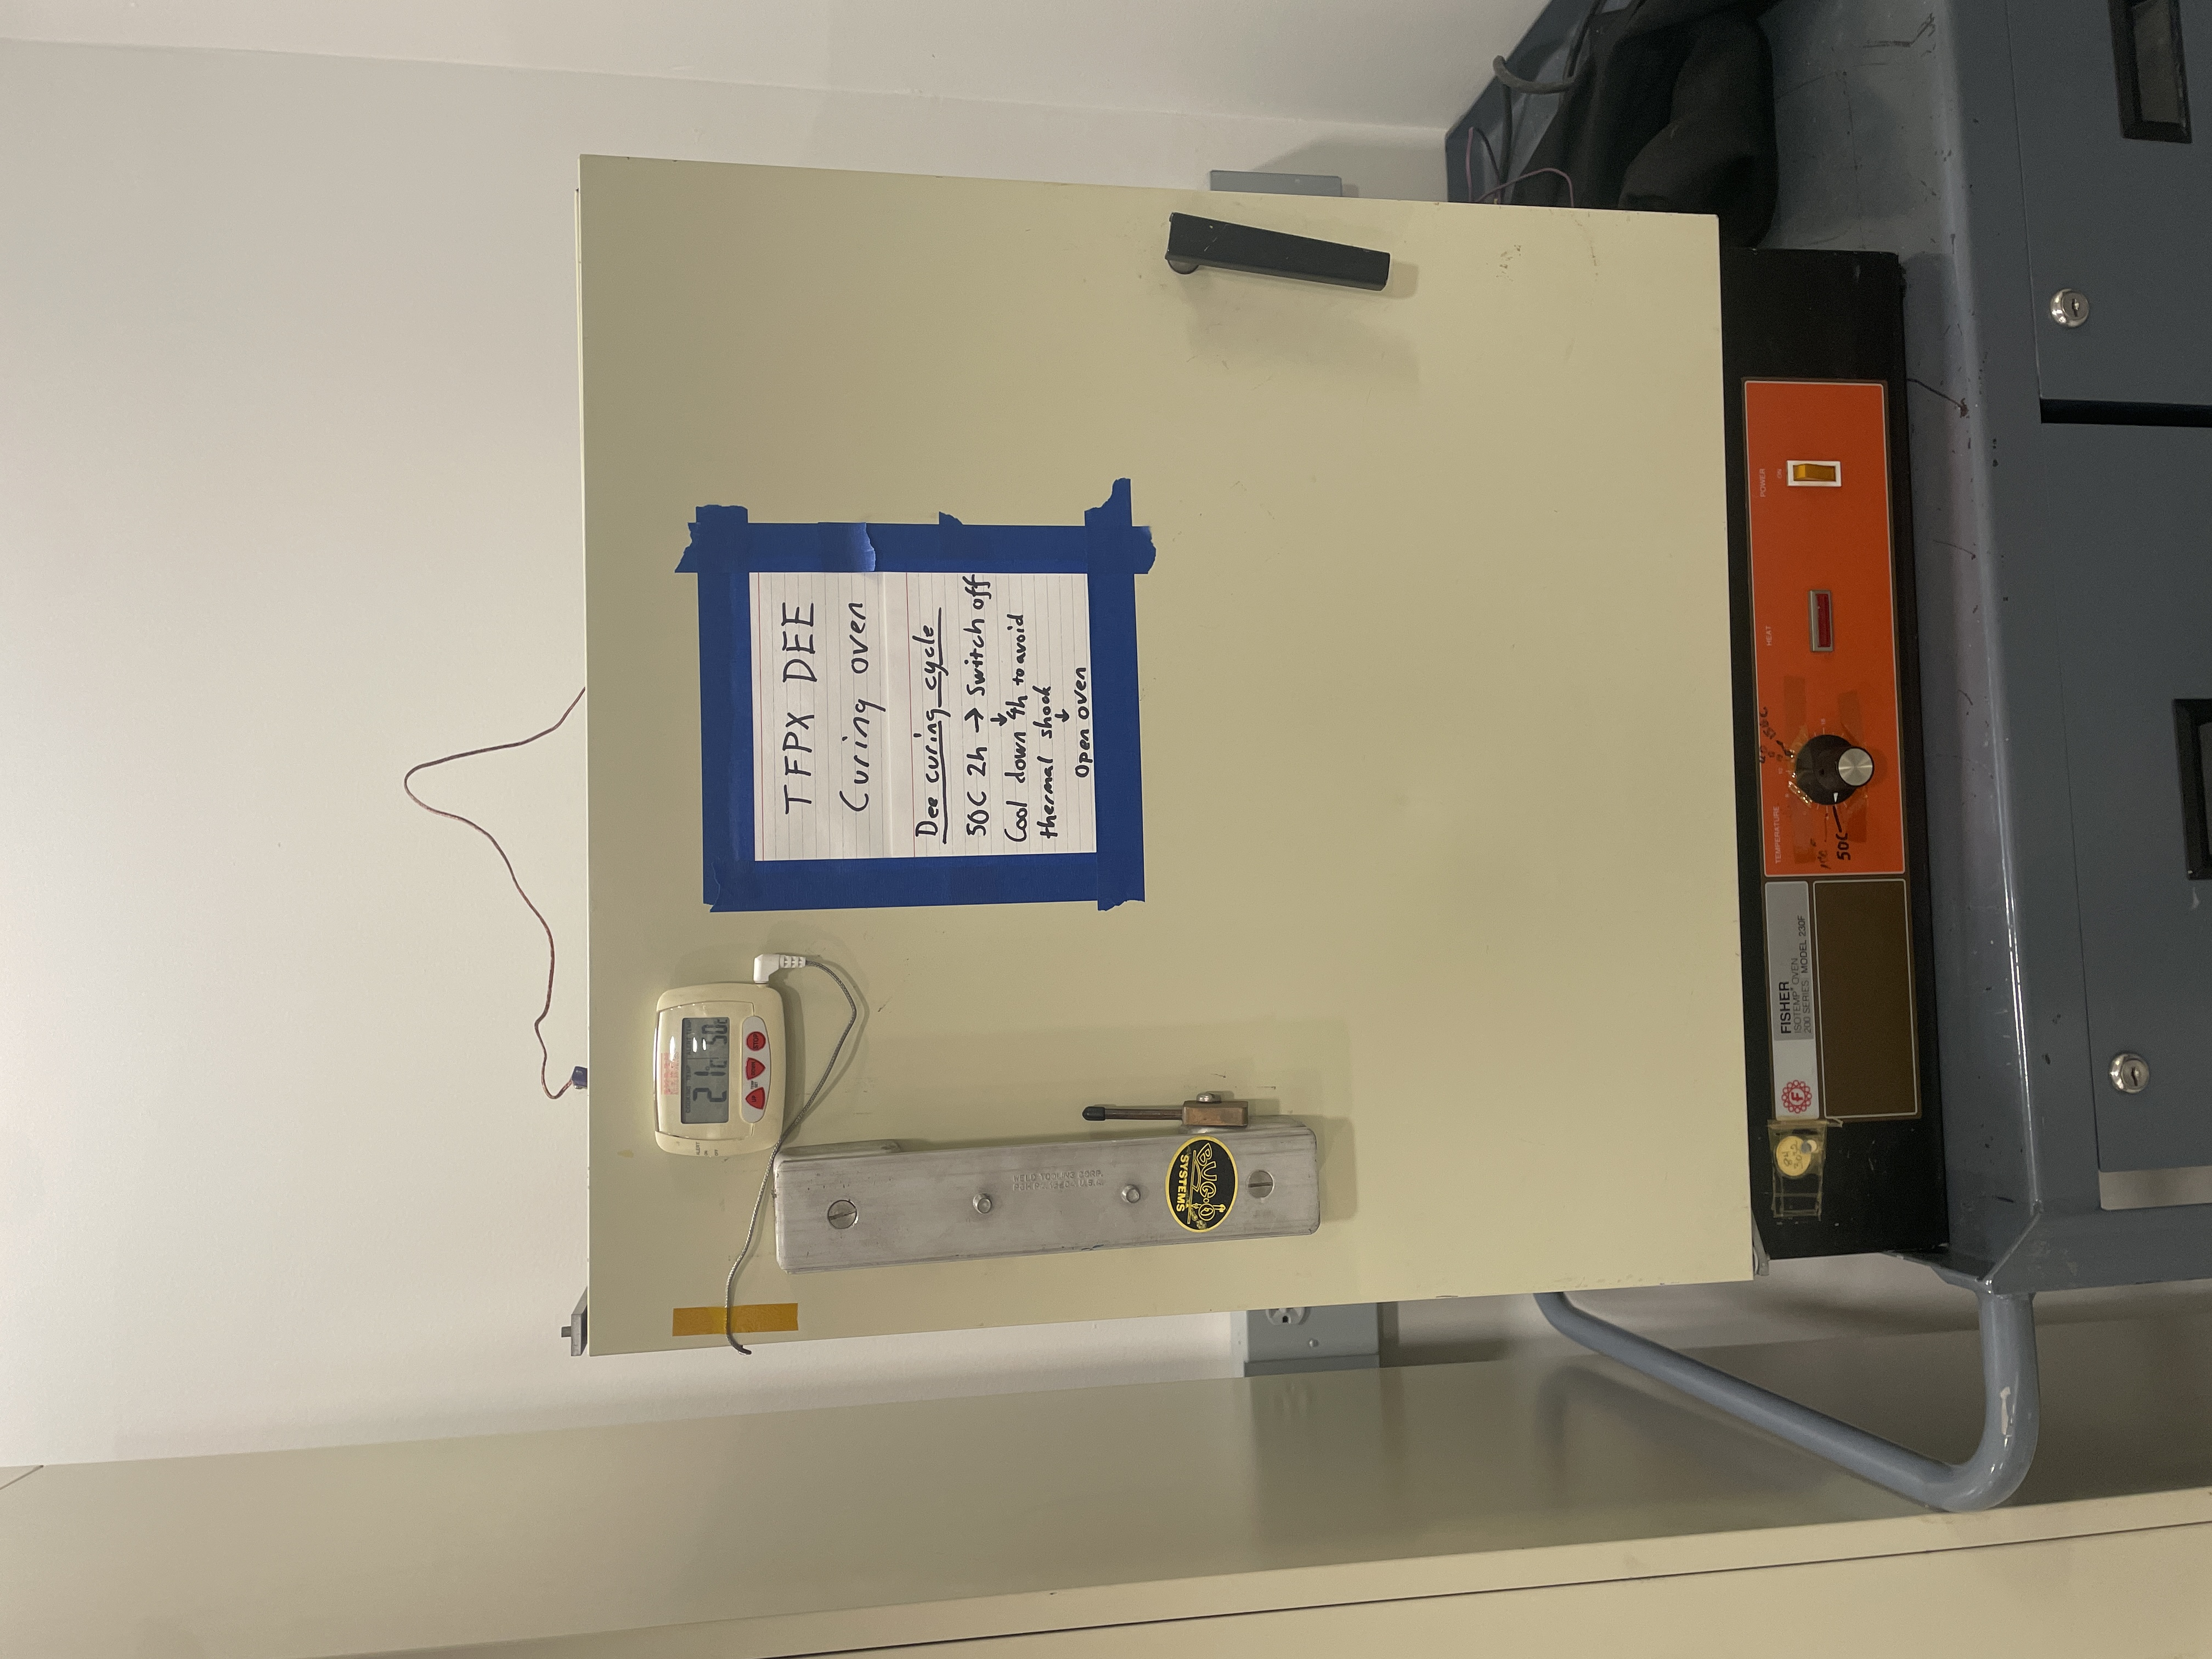
\includegraphics[width=0.9\linewidth, angle=-90]{img/oven.JPG}
            \caption{Oven for curing DEE after assembly}
            \label{oven}
        \end{figure}
        \item Clean up the working space.
%    \end{itemize}
\end{enumerate}
\switchcolumn % Switch to the second column     
\subsubsection*{Person 2:}
\begin{enumerate}
    %Perform a readiness check of epoxy \\preparation area:
%   \begin{itemize}[leftmargin=*]
        \item Ventilate the room with the fan
        \item Put on N95 mask and gloves. Lay out paper towels over the table.
        \item Materials are on the table.
        \item Turn scale on
        \item Check that centrifuge is ready to use.        
%    \end{itemize}      
    %\item Epoxy Mixing and Syringe Preparation
%    \begin{itemize}[leftmargin=*]
        \item Determine the amount of epoxy to be prepared using table in figure \ref{fig:epoxy_calc}.
        A calculator has been set up \href{https://cornellprod.sharepoint.com/:x:/r/sites/TFPXDeemanufacturing/_layouts/15/Doc.aspx?sourcedoc=%7B1955F9BA-B34C-40AF-83B5-E2F571FD91B1%7D&file=Epoxy%20mixing%20calculator.xlsx&action=default&mobileredirect=true}{here} in case a different amount of epoxy is desired. 35g of epoxy is used as reference in the following.
            \begin{center}
            \begin{figure}[h!]
                \centering
                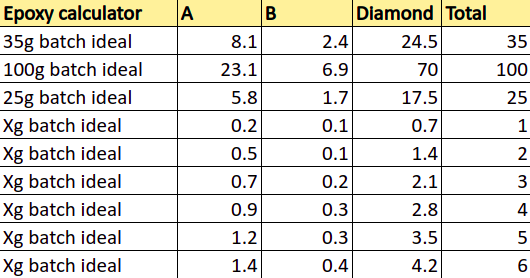
\includegraphics[width=0.8\linewidth]{img/epoxy_calc.png}
                \caption{Epoxy calculator table}
                \label{fig:epoxy_calc}
            \end{figure}
        \end{center}
        \item Place the beaker on the scale and zero the scale. Add 8.1g of Part A using one side of the Popsicle stick.
        \item Zero the scale again. Add 2.4g of Part B using the other side of the stick.
        \item \textbf{Communicate with Person 1 to start the LabView program to set a timer for the mixing process. Wait for confirmation.}       
        \item Add 24.5g of diamond powder and mix until a uniform grayish-green\\ consistency is achieved.
        \item Prepare the syringe, don't forget to put the blue tip cap before centrifuging. Transfer the mixed epoxy into the syringe, ensuring minimal loss.
        \item Centrifuge the syringe for 30 seconds at 2000 RPM.
        \item Ensure no bubbles remain inside the epoxy after centrifugation. If bubbles are present, repeat centrifugation. 
        \item Push the white plastic piston down into the syringe using a sharpie/pen, making sure that the trapped air is removed. 
        \item Take the Epoxy filled syringe to clean room. Pass it to Person 1.
        \item get dressed to get into the clean room   
%    \end{itemize}
    %Evaporator and inserts installation
%    \begin{itemize}
        \item Prepare inserts and Evaporator.
        \item Once the epoxy deposition on stand 2 starts, move bottom jig from stand 1 to working table on the left of gantry. 
        \item Take inserts and stick them on the  CFF\_A carbon foam holes using the tweezers. Be careful not to break/damage the carbon foam.
        \item Insert the evaporator into the groove making sure that it fits. Push with gently with fingers.
        \item Spread plain epoxy over the top surface of the PEEK periphery using the paint brush, so that when CFF\_B is stacked, the carbon fiber sticks to the periphery.  
        \item Prepare top jig plate to complete the full stack.
        \item Clean up the working space.
%    \end{itemize}
\switchcolumn % Switch back to Person 1's tasks:                                           
\end{enumerate}
\end{paracol}

%------------------------------------------------------------------
\section{Documentation}

Any special observations, e.g. damage to parts not already recorded during visual inspection, deviations from normal procedures, should be added to the report in the last step of the routine in the comments pop-up window 

The following information is recorded in the report generated by the gluing software:
\begin{itemize}
    \item Date, time (start--end) and operator name
    \item LabView software: version
    \item Id of parts used:
	\begin{itemize}
	    \item Carbon fiber-foam: S/N
	    \item DEE ID
	    \item Epoxy information
	\end{itemize}
    \item observations/comments
\end{itemize}

Find the report at C:\Users\co2_ctl\Documents\Final_Dee_Assembly\Dee_Assy_Reports\Report.xls path to report. Write an ELog entry or upload the report to the appropriate DataBase.  

\end{document}

